\chapter{Aceptabilidad física: una alternativa}

\noindent El problema planteado al final del capítulo anterior se puede sintetizar como: no hay suficientes mediciones con la precisión necesaria para identificar la EOS de las estrellas de neutrones unívocamente. En este trabajo se explorará si los requerimientos de consistencia física y estabilidad existentes para modelos de estrellas de neutrones pueden ser útiles para complementar las restricciones observacionales.

Acorde con lo anterior, en este capítulo se desarrollarán las herramientas para crear modelos de estrellas de neutrones estáticas. Seguido de esto se enunciarán las condiciones de aceptabilidad física como los requerimientos mínimos que los modelos obtenidos con cualquier EOS debe cumplir.
%\noindent Explicar la variada fenomenología descrita en el capítulo anterior ha requerido la solución de retos teóricos en ramas tan variadas como la relatividad general, física de la materia condensada y física nuclear. 

%En este capítulo se derivarán las ecuaciones de estructura estelar para una estrella de neutrones fría, neutra, estática y con simetría esférica en la teoría newtoniana y en relatividad general. Después de identificar la necesidad de conocer la EOS de la materia para crear modelos estelares, se  describirá el problema de la EOS de la materia ultradensa y algunos de los métodos usados para hallarla.
%Comparar los dos resultados permitirá identificar algunas de las predicciones de la relatividad general en objetos compactos. 
%Para terminar se enunciará una lista de criterios de consistencia física y estabilidad que los modelos estelares deben cumplir, estos criterios serán usados el siguiente capítulo para evaluar qué tan realistas son los modelos estelares obtenidos con diferentes EOSs.


\section{Modelando de estrellas de neutrones estáticas}

\noindent En esta sección se obtendrán las ecuaciones de estructura estelar para una estrella de neutrones fría, neutra, estática y con simetría esférica en la teoría newtoniana y en relatividad general. Comparar los dos resultados permitirá identificar algunos de los efectos que la relatividad general predice en objetos compactos.

\subsection{Caso newtoniano}

\noindent Considerando una distribución de materia con simetría esférica, si $r$ denota la distancia desde el centro de la configuración, la masa encerrada en una superficie esférica de radio $r$ será:  
\begin{equation}
    m ( r ) = \int _ { 0 } ^ { r } 4 \pi r ^ { 2 } \rho \dd{r} = \int_{0}^{r} \dd{m(r)} \quad\text{con}\quad \dd{m(r)}=4\pi r^2\rho \dd{r},
    \label{mN}
\end{equation}
\begin{equation}
    \Longrightarrow\dv{m(r)}{r} =4\pi r^2 \rho.
    \label{dmnewton}
\end{equation}
Ahora, se considera un cilindro infinitesimal a una distancia $r$ del centro, de altura $\dd{r}$ y sección transversal $\dd{A}$, normal al vector posición $\vec{r}$ (ver Figura \ref{stellnew}).  

Si la presión en $\vec{r}$ es $P$ y su cambio al ir de $\vec{r}$ a $\vec{r}+\dd{\vec{r}}$ es $\dd{P}$. La diferencia de presión representa una fuerza 
\begin{equation*}
    F_{Pelem}=-\dd{P}\dd{A},
\end{equation*}
actuando sobre el elemento de masa.

\begin{figure}[H]
    \centering
    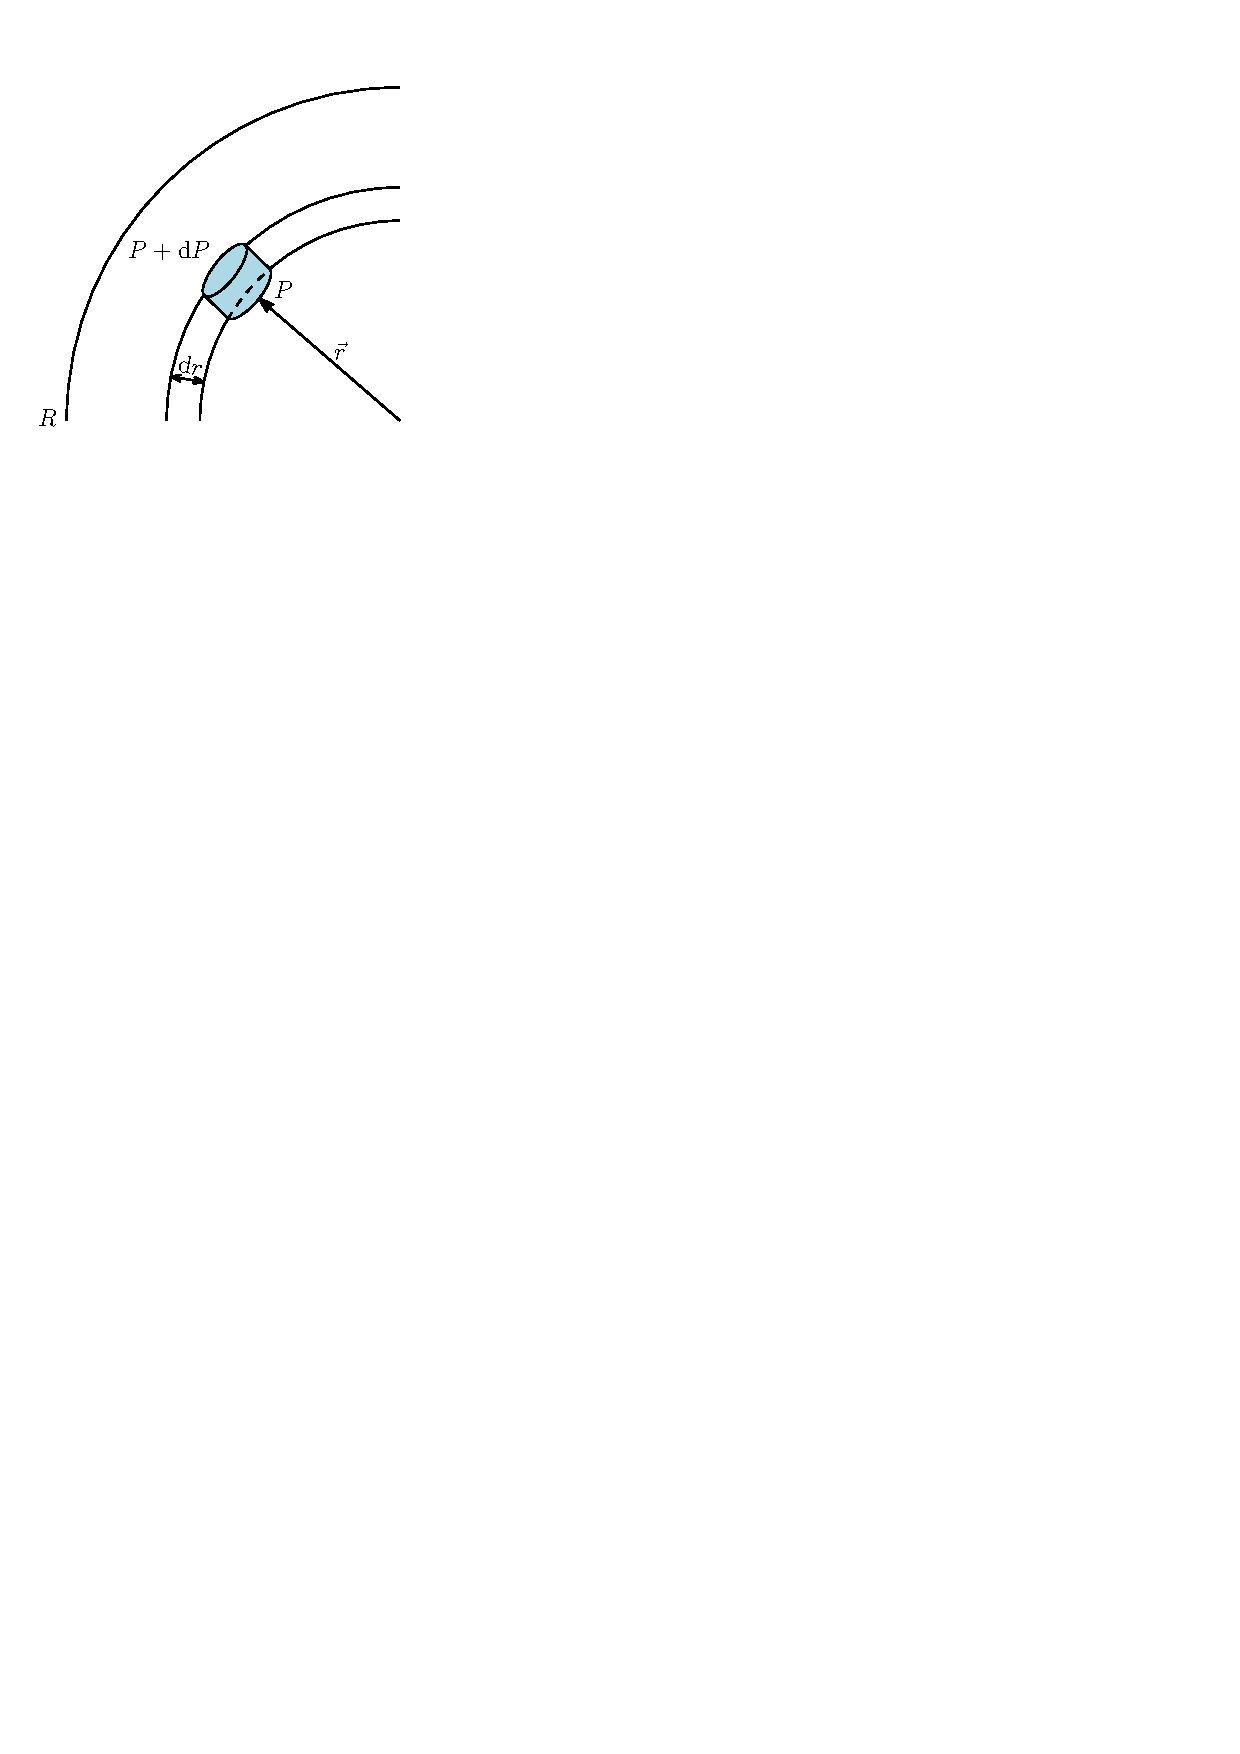
\includegraphics[width=150pt]{figures/stellarnewton.pdf}
    \caption[Presión sobre un elemento de masa cilíndrico]{Presión sobre un elemento de masa cilíndrico.}
    \label{stellnew}
\end{figure}
 Esta fuerza debe contrarrestar la atracción gravitacional sobre el elemento de masa debido a $m(r)$
\begin{equation*}
    F_{atracc}=\frac{G m(r)\rho \dd{A} \dd{r}}{r^2}.
\end{equation*}
Para que el elemento de masa se encuentre en equilibrio se requiere entonces:

\begin{equation}
    -\dd{P}\dd{A} =\frac{G m(r)\rho \dd{A} \dd{r}}{r^2},
\end{equation}
o
\begin{equation}
    \dv{P}{r} = - \frac { G m ( r ) } { r ^ { 2 } } \rho.
    \label{dpnewton}
\end{equation}
que es la conocida ecuación de equilibrio hidrostático. 

Las ecuaciones \eqref{dmnewton} y \eqref{dpnewton} son las ecuaciones de estructura estelar newtonianas \cite{Chandrasekhar1958}. 

%Si una relación entre la presión y la densidad $P(\rho)$ es dada, es decir, una ecuación de estado, el sistema puede resolverse dado un par condiciones iniciales $m(r=0)$ y $P(r=0)$. La primera de estas condiciones es evidente puesto que no hay masa encerrada en un cascarón esférico de radio nulo, $m(r=0)=0$. La segunda estará definida por el valor de $\rho(r=0)\equiv\rho_c$ escogido, mediante la ecuación de estado, $P(r=0)=P(\rho_c)$.

%El radio de la estrella $R$ se define como el valor de $r$ en el que la presión se anula, esto es, $P(R)=0$ y de manera similar la masa de la estrella $M$ se define como el valor de la masa encerrada en $r=R$, esto es, $m(R)=M$.

Aunque no se van a tratar en este trabajo, cabe resaltar que las \emph{enanas blancas}, objetos compactos sostenidos por la presión de degeneración de electrones, pueden ser descritas por las ecuaciones de estructura newtonianas satisfactoriamente. Una manera de conocer la importancia de las correcciones relativistas de una estrella es comparando el valor de la compacidad de la estrella $\mu \equiv \frac{2GM}{c^2R}$ con la unidad (la razón será evidente en el resultado relativista) \cite{Weinberg1972}. Las enanas blancas tienen masas en un rango de $0.33\,M_{\odot}$ $1.52\,M_{\odot}$ y radios típicos de unos cuantos miles de kilómetros \cite{Glendenning2000}. Para una enana blanca promedio, con masa $M=0.6\,M_{\odot}$ y radio $r=3000 \,\rm{km}$ se tiene
\begin{equation}
    \mu \simeq 6\times 10^{-4}\ll 1,
\end{equation}
por lo cual se espera que el tratamiento newtoniano sea suficiente. 

\subsection{Caso relativista}\label{CR}
%\TODO{Basado en los comentarios de la propuesta modificar esta sección. Teniendo en cuenta que los cálculos están hechos en el apéndice.}

%Si bien en la teoría newtoniana podrían existir objetos tan compactos como las estrellas de neutrones, algunas de las predicciones presentan inconsistencias con lo predicho por la teoría de la Relatividad General. Por ejemplo, Chandrasekhar encontró (usando gravedad newtoniana) que las estrellas soportadas por presión de degeneración tienen una masa máxima, obtenida asintóticamente cuando los fermiones son altamente relativistas. Esto es, cuando tienen velocidades comparables con la velocidad de la luz. Bajo tales condiciones la teoría newtoniana permitiría la existencia de estrellas compuestas por los quarks más pesados (charm, bottom y top). En Relatividad General se predice también la existencia de una masa máxima, pero ésta no es de naturaleza asintótica sino que está inmersa en la forma de las ecuaciones de estructura estelar. Las estrellas con la mayor masa posible en Relatividad General, en contraste a lo predicho por la teoría newtoniana, no son lo suficientemente densas para permitir la presencia de los quarks más pesados \cite{Glendenning2000}.

%Predicciones contradictorias como la anterior favorecen a la Relatividad General en el estudio de objetos compactos, pues ésta ha explicado fenómenos como la precesión de mercurio, que no pueden ser explicados en gravedad newtoniana (ver  \cite{Turyshev2008ExperimentalRelativity} para una revisión de tests experimentales de la Relatividad General).

\noindent\small{\textbf{Nota:} a lo largo de esta sección se hará uso del convenio de suma de Einstein y de unidades gravitacionales ($G=c=1$), excepto en donde sea explícitamente especificado. Además, las primas representan derivada con respecto a $r$ y se usará esta notación indistintamente con la notación diferencial.}
\normalsize

\noindent Para describir la estructura de una estrella estática en Relatividad General se supone un espacio-tiempo asintóticamente plano, estático y con simetría esférica, descrito de manera general por el elemento de linea:

\begin{equation}
\dd{s}^ { 2 } = -e ^ { 2 \nu ( r ) } \dd{ t} ^ { 2 } + e ^ { 2 \lambda ( r ) } \dd{ r} ^ { 2 } + r ^ { 2 } \left( \dd{ \theta} ^ { 2 } + \sin ^ { 2 }  \theta  \dd{ \phi} ^ { 2 } \right) .   
\end{equation}

Respecto a una base ortonormal
\begin{equation}
    \omega^0=\,e^{\nu}\dd{t}, \quad
    \omega^1=\,e^{\lambda}\dd{r}, \quad
    \omega^2=\,r\dd{\theta}, \quad
    \omega^3=\,r\sen{\theta}\dd{\varphi},
\end{equation}
el tensor de Einstein asociado a este elemento de linea tiene componentes no nulas (ver el Apéndice \ref{curvature} para la derivación)

\begin{equation}
    \begin{array} { l } { G _ { 0 } ^ { 0 } = e ^ { - 2 \lambda } \left( \frac { 1 } { r ^ { 2 } } - \frac { 2 \lambda ^ { \prime } } { r } \right) - \frac { 1 } { r ^ { 2 } }  }, \\ { G _ { 1 } ^ { 1 } = e ^ { - 2 \lambda } \left( \frac { 1 } { r ^ { 2 } } + \frac { 2 \nu ^ { \prime } } { r } \right) - \frac { 1 } { r ^ { 2 } } }, \\ { G _ { 2 } ^ { 2 } = e ^ { - 2 \lambda } \left( \nu ^ { \prime \prime } + \nu ^ { \prime 2 } - \lambda ^ { \prime } \nu ^ { \prime } + \frac { \nu ^ { \prime } - \lambda ^ { \prime } } { r } \right)  }, \\ { G _ { 3 } ^ { 3 } = G _ { 2 } ^ { 2 }  }, \end{array}
    \label{eee}
\end{equation}

debe satisfacer las ecuaciones de Einstein
\begin{equation}
    G _ { \mu } ^ { \nu }  = 8 \pi T _ { \mu } ^ { \nu },
\end{equation}
fijando así las funciones métricas $\nu$ y $\lambda$, en función del contenido material de la estrella descrito por $T _ { \mu } ^ { \nu }$.

Dividiendo el espacio-tiempo en dos: una región exterior a la estrella y una interior. 
La \textit{región exterior} no tiene fuentes ($T _ { \mu } ^ { \nu }=0$) y las ecuaciones de Einstein para ésta son 
\begin{equation}
    G _ { \mu } ^ { \nu } = 0.
\end{equation}
Este es un sistema de 3 ecuaciones, pues $ G _ { 2 } ^ { 2}=G _ { 3 } ^ { 3}$ y dos incógnitas ($\nu$ y $\lambda$). Las identidades de Bianchi aseguran que una las ecuaciones puede ser escrita en términos de las otras y no brinda información adicional.

Este sistema puede ser resuelto de manera sencilla para obtener (ver el Apéndice \ref{curvature} para una derivación)
\begin{align}
    e^{2\nu}=e^{-2\lambda}=1-\frac{2 M}{r},
\end{align}


que es la conocida solución exterior de Schwarzschild
\begin{equation}
    \dd{s} ^ { 2 } = - \left( 1 - \frac { 2 M } { r } \right) \dd{t} ^ { 2 } + \left( 1 - \frac { 2 M } { r } \right) ^ { - 1 } \dd{r} ^ { 2 }  + r ^ { 2 } \dd{\theta} ^ { 2 } + r ^ { 2 } \sin ^ { 2 } \theta \dd{\phi} ^ { 2 }, \label{schwarzs}
\end{equation}
valida para $r>R$, donde $R$ es el radio de la estrella y $M$ es una constante de integración, que puede ser interpretada como la masa gravitacional al comparar con el límite de campo débil. Este elemento de línea describe la geometría del espacio-tiempo exterior a una estrella estática.

\begin{figure}%[H]
    \centering
    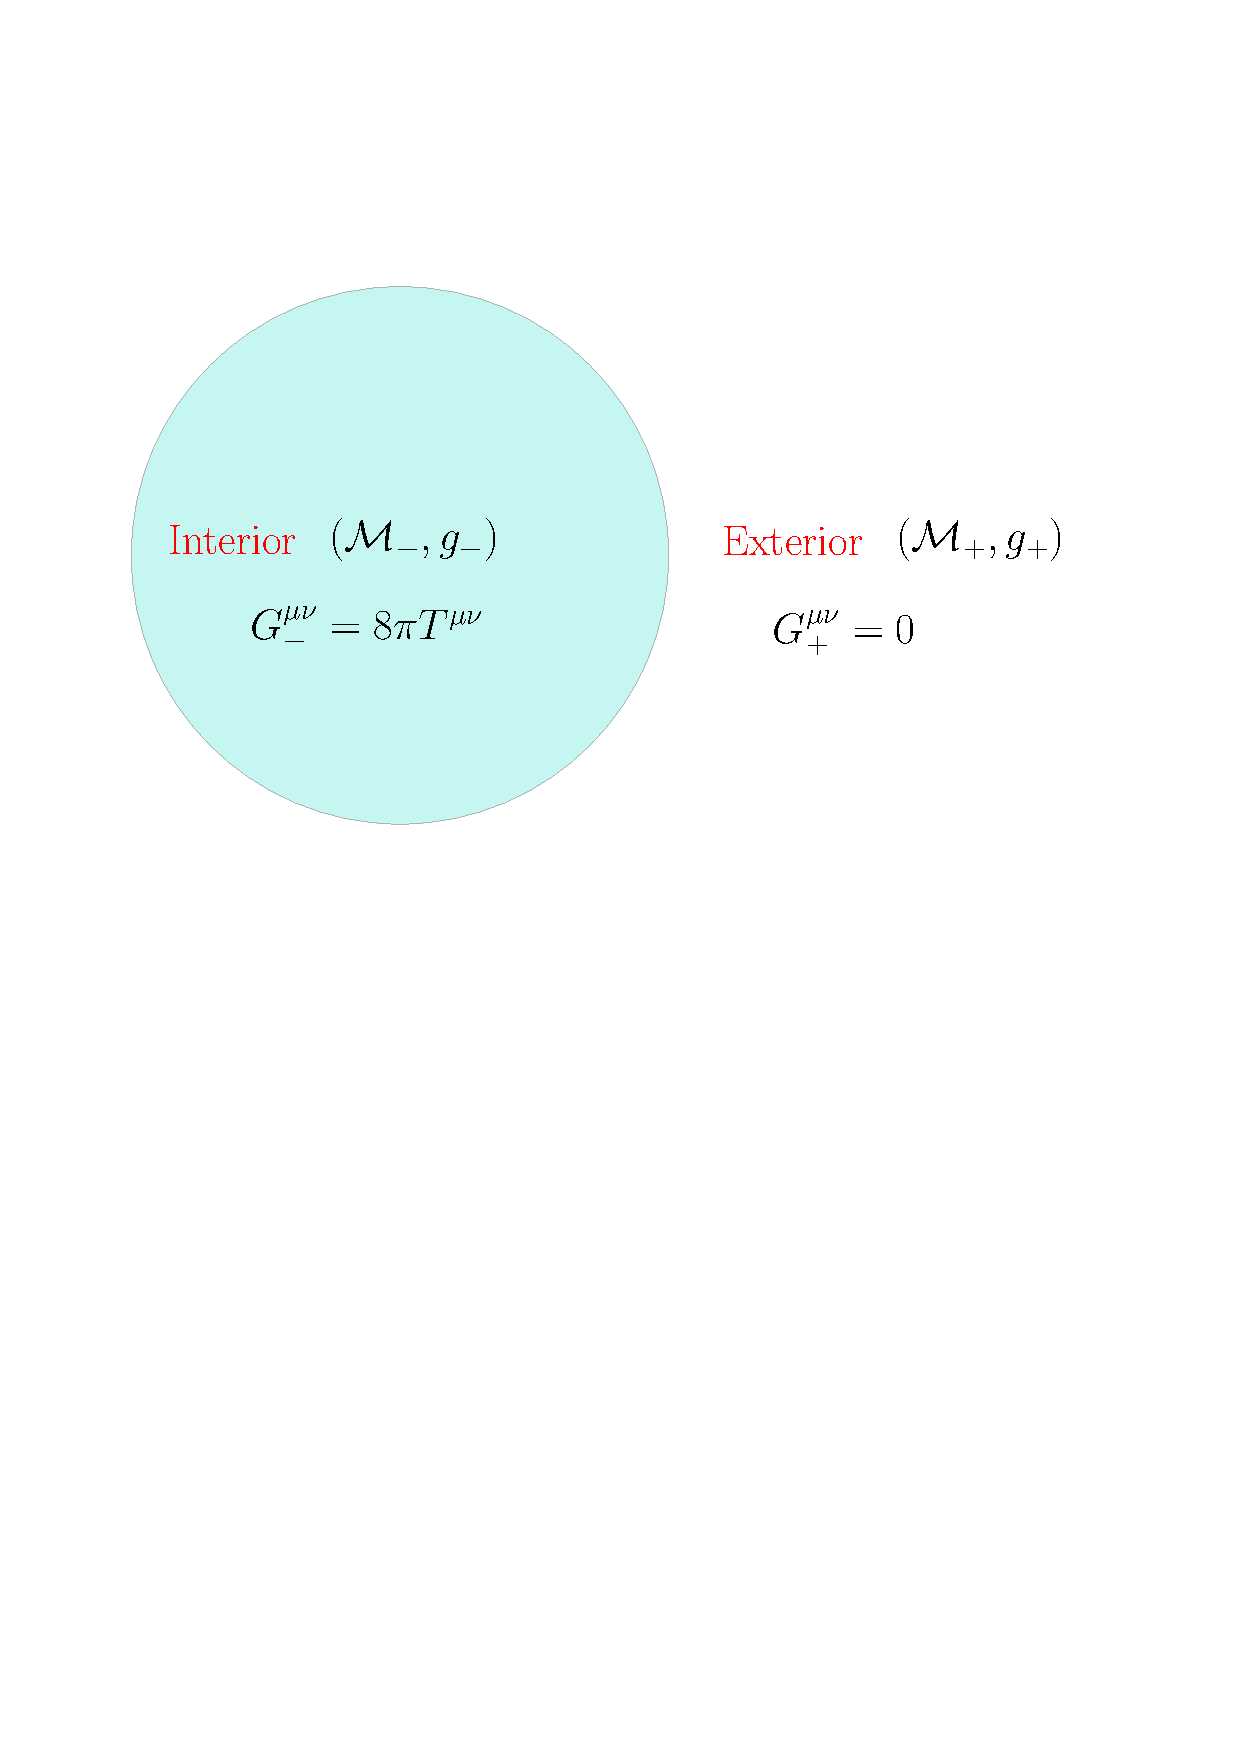
\includegraphics[width=0.7\linewidth]{figures/GR.pdf}
    \caption[División del espacio-tiempo]{División del espacio-tiempo en un espacio-tiempo exterior y un interior. Al asumir que ambos espacio-tiempos son estáticos y tienen simetría esférica las métricas $g_{-}$ y $g_{+}$, así como los tensores de Einstein $G^{\mu \nu}_{-}$ y $G^{\mu \nu}_{+}$ tienen la misma forma.}
    \label{STDiv}
\end{figure}

Para la \textit{región interior} el contenido material debe ser especificado para resolver las ecuaciones de Einstein. Si la materia se modela como un fluido perfecto, el tensor de energía-momento viene dado por

\begin{equation}\label{EMT}
    T ^ { \mu \nu } =  P g ^ { \mu \nu } + ( P + \rho ) u ^ { \mu } u ^ { \nu }
\end{equation}

donde $u^{\mu}=\dv{x^{\mu}}{\tau}$ es la cuadri-velocidad de modo que $g _ { \mu \nu } u ^ { \mu } u ^ { \nu } = -1$ , $P$ su presión y $\rho$ su densidad de energía ambas definidas en un marco comóvil al fluido. Este tensor de energía-momento puede ser deducido del Lagrangiano $L=-\rho$ usando el principio variacional \cite{Felice19992}.

Como se considera una estrella estática, la velocidad espacial de todos los elementos del fluido es cero:
\begin{equation}
    u^{i}=0 \quad (i=1,2,3)\qc u ^ { 0 } = 1
\end{equation}
con lo que las únicas componentes no nulas del tensor energía-momento, en componentes mixtas, serán
\begin{equation}
T _ { 0 } ^ { 0 } = -\rho(r) , \quad T _ { i } ^ { i } =  P(r) \quad ( i=1,2,3 ).  
\end{equation}
Con esta forma del tensor energía-momento y las componentes del tensor de Einstein enunciadas anteriormente, las ecuaciones de Einstein son
\begin{align}
     e ^ { - 2 \lambda } \left( \frac { 1 } { r ^ { 2 } } - \frac { 2 \lambda ^ { \prime } } { r } \right) - \frac { 1 } { r ^ { 2 } } =&  -8\pi\rho, \label{E00} \\
    e ^ { - 2 \lambda } \left( \frac { 1 } { r ^ { 2 } } + \frac { 2 \nu ^ { \prime } } { r } \right) - \frac { 1 } { r ^ { 2 } } =& \, 8\pi P, \label{E11}\\
    e ^ { - 2 \lambda } \left( \nu ^ { \prime \prime } + \nu ^ { \prime 2 } - \lambda ^ { \prime } \nu ^ { \prime } + \frac { \nu ^ { \prime } - \lambda ^ { \prime } } { r } \right) =& \, 8\pi P. \label{E22}
\end{align}

Este sistema de ecuaciones puede ser escrito en una manera más sencilla de integrar usando las Ecuaciones \eqref{E00} y \eqref{E11} suplementadas con la conservación local de la energía y el momento
\begin{equation}
    \qty(\nabla_{\omega_\nu}\mathbf{T})^{\mu \nu} = 0 \label{CEM}.
\end{equation}
La Ecuación \ref{E22} no aportará nueva información pues las identidades de Bianchi aseguran que esta ecuación es una consecuencia de las Ecuaciones \eqref{E00},\eqref{E11} y \eqref{CEM} \cite{Schutz2009}.

Definiendo la variable 
\begin{equation}
     m(r) \equiv \frac{1}{2}r\qty(1-e^{-2\lambda}), \label{misnermass}
\end{equation}
las ecuaciones \eqref{E00}, \eqref{E11} y \eqref{CEM} se reducen al sistema de ecuaciones 
\begin{subequations}
\begin{align}
    \dv{m}{r} &= 4\pi \rho r^2, \label{dmtov} \\
     \dv{P}{r} &= -(P+\rho)\frac{m+4\pi P  r^3}{r\qty(r-2m)},\label{dptov} \\
    \dv{\nu}{r} &= \frac{m+4\pi P   r^3}{r\qty(r-2m)}.\label{dnutov}
\end{align}
\end{subequations}
Las ecuaciones \eqref{dmtov}, \eqref{dptov} y \eqref{dnutov} son las ecuaciones de estructura estelar relativista: describen configuraciones de estrellas de neutrones estáticas en equilibrio. Este sistema de ecuaciones se conoce generalmente como las ecuaciones de Tolman-Oppenheimer-Volkoff (TOV)  \cite{Tolman1939,Oppenheimer1939} y serán referidas de esta manera en adelante. 

Re-escribiendo \eqref{dptov} en unidades SI como
\begin{equation}
    \dv{P}{r} =  - \frac { G  m ( r ) } { r ^ { 2 } } \rho ( r ) \left[ 1 + \frac { P ( r ) } {c ^ { 2 } \rho ( r ) } \right] \left[ 1 + \frac { 4 \pi r ^ { 3 } P ( r ) } { m ( r ) c ^ { 2 } } \right]  \left[ 1 - \frac { 2 G m ( r ) } { c ^ { 2 } r } \right] ^ { - 1 }, 
    \label{dprelat}
\end{equation}
se aprecia que la versión relativista añade correcciones a la ecuación de equilibrio hidrostático newtoniana \eqref{dpnewton} en forma de tres factores adimensionales. Las dos versiones de las ecuaciones de estructura coinciden cuando estos factores se reducen a la unidad, esto es, en el límite cuando 
\begin{equation}
    c^2\rho \gg P \qc mc^2 \gg 4\pi r^3P \quad \text{y} \quad  \frac{2Gm}{c^2r}= \mu \ll 1,
\end{equation}
en un límite no relativista la variable $m$ definida en \eqref{misnermass} (conocida como masa gravitacional)  coincide con la masa Newtoniana \eqref{mN}, además $P$ y $\rho$ varían como $\frac{1}{2}mv^2$ y  $mc^2$ \cite{Silbar2003}. Así, las dos primeras correcciones son de orden $v^2/c^2$ y son válidas cuando las partículas del fluido tienen velocidades pequeñas comparadas con la velocidad de la luz mientras el tercer factor es puramente geométrico. 

Debido a que los tres factores en la ecuación \eqref{dprelat} son mayores que 1, si se compararan dos modelos estelares: uno Newtoniano y otro relativista, que para cierto radio $r$ tienen los mismos valores de $\rho$, $P$ y $m$, la relatividad general predice fuerzas gravitacionales más fuertes sobre la estrella que la teoría Newtoniana. Esto tiene un efecto importante en la estabilidad pues, como se discutirá en la sección \ref{phyacep}, configuraciones que eran estables en la teoría Newtoniana no lo serán en relatividad general. 
%Así pues,  \eqref{dprelat} expresa el \textit{balance} entre la fuerza neta sobre un elemento de masa debido a la presión de la materia que la rodea y la atracción gravitacional de la materia interior a este. Los tres factores en la ecuación \eqref{dprelat} son mayores que 1, esto es, además de la densidad de energía, la presión actúa como una fuente de atracción gravitacional. Esta es la razón por la cual el colapso gravitacional es intrínseco a la estructura de la Relatividad General: mientras en las estrellas newtonianas la presión actuaba para sostener a la estrella, si la estrella es lo suficiente masiva (presiones lo suficientemente grandes) el colapso es inevitable.

\subsection{Cómo construir modelos estelares.}\label{SMABC}

\noindent Las ecuaciones de TOV
\begin{align*}
    \dv{m}{r} &= 4\pi \rho r^2, \\
    \dv{P}{r} &= -(P+\rho)\frac{m+4\pi P r^3}{r\qty(r-2m)}, \\
    \dv{\nu}{r} &= \frac{m+4\pi P r^3}{r\qty(r-2m)},
\end{align*}
son un sistema de tres ecuaciones diferenciales ordinarias con cuatro incógnitas $m(r)$, $\rho(r)$, $P(r)$ y $\nu(r)$. Para solucionar este sistema se necesita una ecuación más: la ecuación de estado (EOS) de la materia en la estrella que se puede expresar generalmente como una relación $P=P(\rho)$. 

Dada una ecuación de estado $P(\rho)$, \emph{un modelo estelar está completamente definido por el valor de la densidad central} $\rho(r=0)=\rho_c$. Esto se debe a que dado $rho_c$ el resto de condiciones iniciales ya están especificadas: usando la ecuación de estado se obtiene $P(r=0)=P(\rho_c)$, por definición $m(r=0)=0$ y $\nu(r=0)$ es una constante arbitraria que se renormalizará para cumplir las condiciones de acoplamiento. Con los valores iniciales especificados, el sistema acoplado se puede integrar desde $r=0$ hasta que la presión se anule, lo que indica el borde de la estrella y define el radio $R$ y la masa gravitacional $m(R)=M$ de la estrella. 

%Si la materia de la estrella de neutrones se supone como compuesta por un conjunto $B$ de bariones ($B=n,p,\Sigma^{-},\Lambda,...$), la dificultad de hallar la ecuación de estado reside en calcular la energía del estado base por barión del sistema:
%\begin{equation}
%    E_{\mathrm{B}}=\frac{\left(\Psi_{0}\left|\hat{H}_{\mathrm{B}}\right| \Psi_{0}\right)}{A_{\mathrm{b}}\left(\Psi_{0} | \Psi_{0}\right)},
%\end{equation}
%donde $\hat{H}_B$ es el operador Hamiltoniano de la especie bariónica $B$ y $\psi_0$ es la ecuación de onda del estado base del sistema, en términos de las densidades de bariones $n_B$. A partir de la cual se puede calcular la ecuación de estado \cite{Haensel2007NeutronStructure}. 

%Los diversos modelos de ecuaciones de estado obtienen $E_B({n_B})$ mediante diferentes métodos, los cuales se pueden agrupar en cuatro categorías: modelos de Brueckner-Hartree-Fock, modelos basados en el método variacional,  modelos basados en un funcional de densidad de energía y modelos de teoría de efectiva de campos. 

%A continuación se presentarán algunos detalles de cada uno de estos enfoques.\TODO{Sacar los resúmenes del Pokethin.}
%\subsection{Modelos de Brueckner-Hartree-Fock}

%\subsection{Modelos de métodos variacionales}

%\subsection{Modelos de funcionales de densidad de energía}

%\subsection{Modelos de teoría de campos relativista}


\section{Condiciones de aceptabilidad física}\label{phyacep}
\noindent Para que los modelos de objetos compactos obtenidos sean de interés astrofísico, las variables físicas y métricas deben cumplir con varias condiciones de regularidad, acoplamiento y estabilidad. Estas condiciones fueron recopiladas recientemente por B. V. Ivanov \cite{Ivanov2017} y extendidas por Nuñez et al. \cite{Hernandez2018}, a continuación se presentará la lista de condiciones y el fundamento físico de cada una.

\subsection*{Sobre los potenciales métricos.}
\noindent Las componentes del tensor métrico $\tensor{g}{_\alpha_\beta}$ reciben el nombre de potenciales métricos por la cercana relación que $\tensor{g}{_0_0}$ tiene con el potencial gravitacional Newtoniano $\phi$, en el límite de campo débil. Como el principio de equivalencia requiere que la métrica tenga una signatura $+2$, esto es, que en cada punto $\tensor{g}{_{alpha}_{\beta}}$ sea reducible a diag($-1,1,1,1$), generalmente se fija el signo de las componentes diagonales de la métrica acordemente: ($-, +, +, +$). Debido a esto se requiere que los potenciales métricos no sean negativos, ya que se alteraría la signatura de la métrica.

\textbf{C1:} Los potenciales métricos son positivos y deben ser finitos y libres de singularidades en el interior de la estrella.
\subsection*{Condiciones de acoplamiento.}
\noindent Para acoplar la solución interior y exterior sobre la superficie de la estrella, es necesario imponer condiciones de acoplamiento de modo que el espacio-tiempo esté bien definido. 
La formulación de estas condiciones que será presentada (adaptada de \cite{Misner1973}) fue desarrollada por Darmois \cite{Darmois1927} e Israel \cite{Israel1966} y se basa en consideraciones sobre la curvatura intrínseca y extrínseca de la 3-superficie tipo tiempo $\Sigma$ que describe la superficie de la estrella.
 
 Si $\vec{n}$ es el vector (tipo espacio) normal a $\Sigma$, se introducen coordenadas normales Gaussianas donde $n=cte$ define 3-superficies tipo tiempo vecinas a $\Sigma$ (ver Figura \ref{JC}). La métrica en estas coordenadas tiene la forma 
 \begin{equation}
g=(\vec{n} \cdot \vec{n})^{-1} d n\otimes d n +g_{i j} d x^{i} \otimes d x^{j},
\end{equation}
donde $\tensor{g}{_i_j}$ son los coeficientes métricos de la 3-geometría.  

 \begin{figure}%[H]
     \centering
     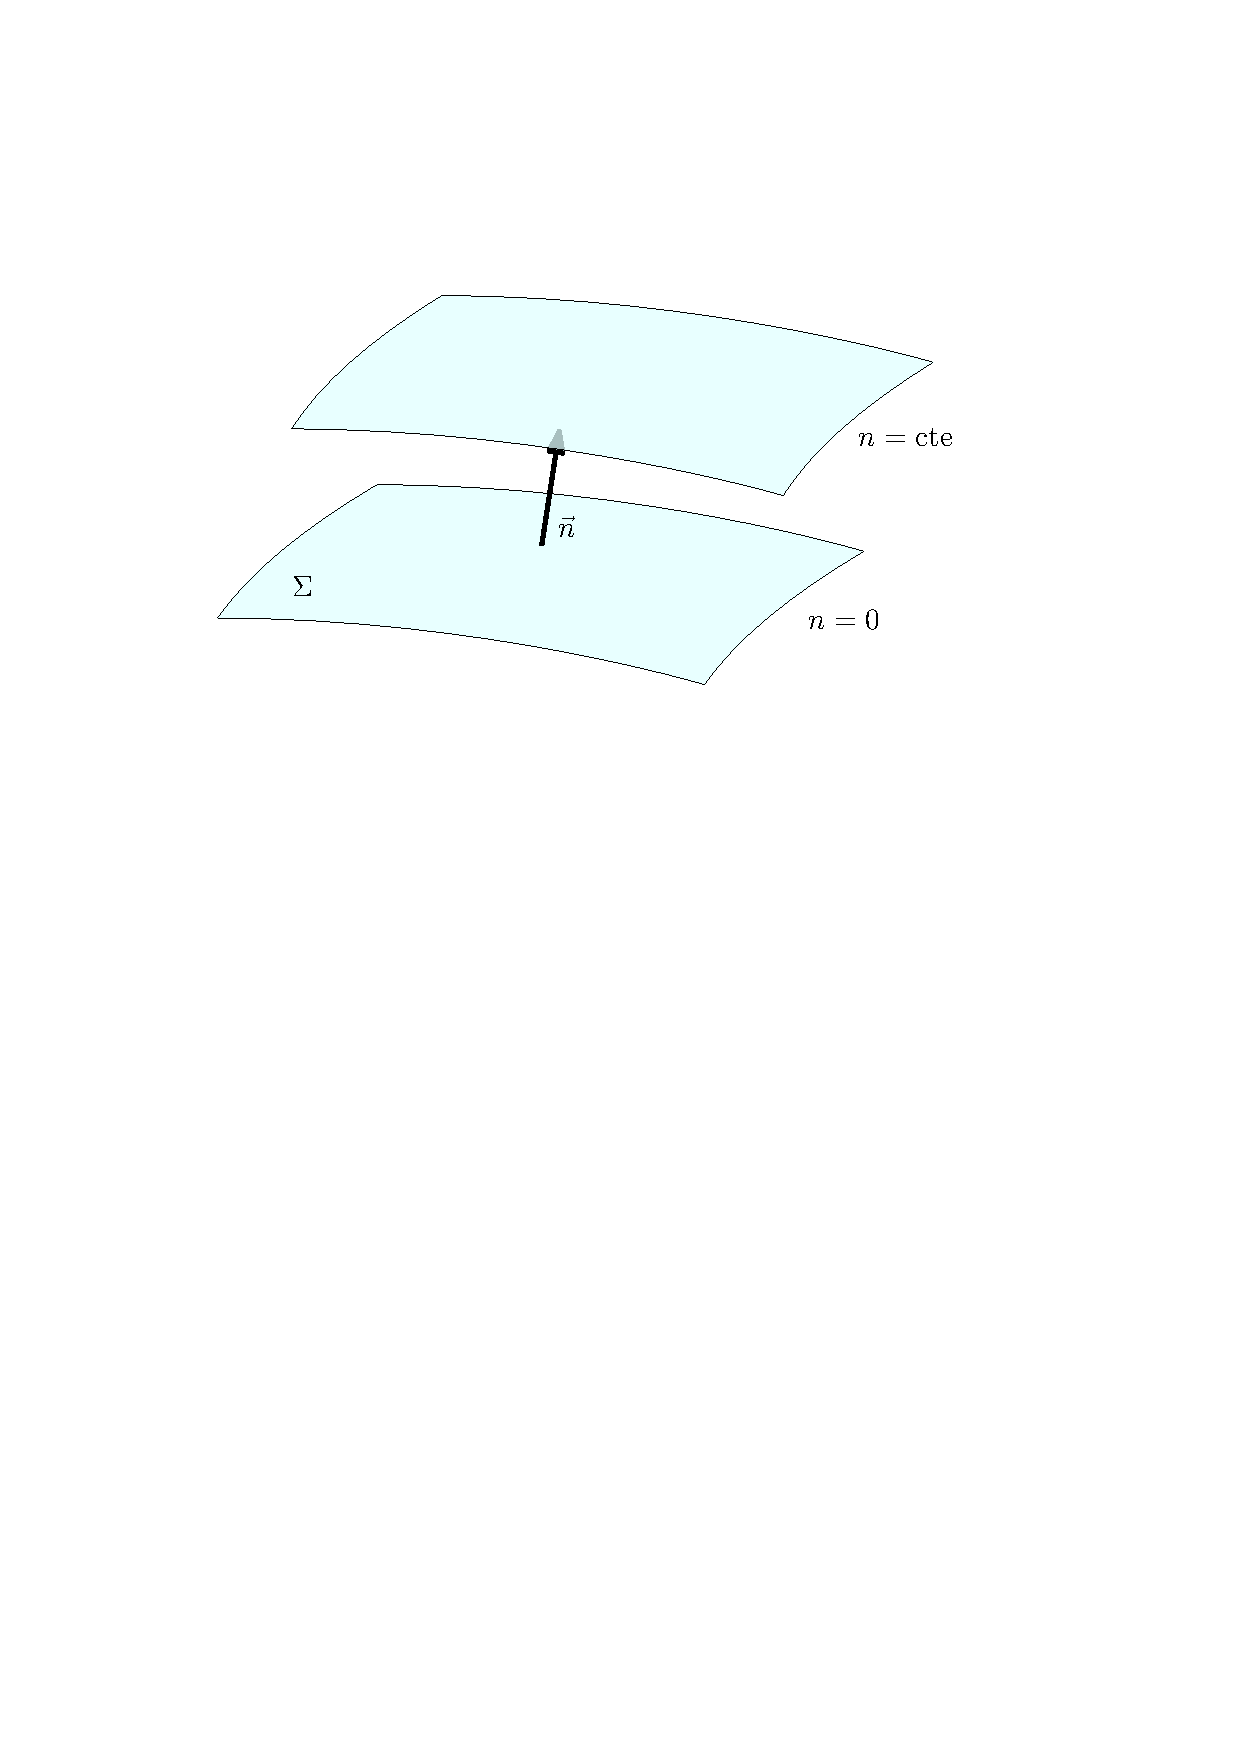
\includegraphics[width=0.7\linewidth]{figures/Junction.pdf}
     \caption{Coordenadas Gausianas en el vecindario a $\Sigma$}
     \label{JC}
 \end{figure}
Si a través de la superficie no hay contenido material, las condiciones de acoplamiento en estas coordenadas son:
 \begin{enumerate}[leftmargin=2cm]
     \item La métrica de las 3-superficies $g_{ij}$ es continua a través de $\Sigma$.
     \item El tensor de energía-momento superficial se anula
     \begin{equation}
\tensor{S}{^\alpha_\beta}\equiv\lim _{\varepsilon \rightarrow 0}\left[\int_{-e}^{+\varepsilon} T_{\beta}^{\alpha} d n\right]=0.
    \end{equation}
 \end{enumerate}

 Como es explicado en \cite{Misner1973} la condición 2 es equivalente a exigir la continuidad de la segunda forma fundamental. 
 
 \textbf{C2:} Para el caso considerado en este trabajo $\Sigma:\,r=R$, además la simetría esférica permite identificar $\vec{n}=\pdv{r}$ y debido a que la métrica exterior es la de Schwarzschild $\eval{T^{\alpha}_{\beta}}_{+\epsilon}$= 0, teniendo en cuenta estas consideraciones las condiciones de acoplamiento se reducen a
 \begin{enumerate}[leftmargin=2cm]
     \item $e ^ {  2 \nu(R) } =  1 - \frac { 2 M } { R }= e ^ { -2 \lambda(R) }$.
    \item $P(R)=\rho(R)=0$.
 \end{enumerate}


\subsection*{ Sobre el corrimiento al rojo gravitacional.}
\noindent La luz emitida por una estrella es observada corrida al rojo por un observador lejano debido a la presencia del campo gravitacional. Qué tanto es corrida al rojo puede ser estimado de manera sencilla con u argumento basado en óptica geométrica \cite{Glendenning2000}: considerando un átomo de la estrella a una distancia $r$ de su centro, que emite un fotones con determinada frecuencia, el intervalo de tiempo propio entre dos emisiones consecutivas está dado por
\begin{equation}
d \tau=\sqrt{-g_{\mu \nu} d x^{\mu} d x^{\nu}},
\end{equation}
en el marco del átomo esto es simplemente ($dx^i=0$)
\begin{equation}
d \tau_{\mathrm{e}}=\sqrt{-g_{00}(r)} d t.
\end{equation}
El intervalo espacio-temporal para un rayo radial será
\begin{equation}
d \tau^{2}=g_{11}(r) d r^{2} - g_{00}(r) d t^{2} = 0,
\end{equation}
así que el tiempo que tardó un pulso en viajar de $r$ a $\infty$ es
\begin{equation}\label{timeinterval}
\Delta t=t_{\infty}-t_{r}= \int_{r}^{\infty}\left(\frac{g_{11}(\bar{r})}{g_{00}(\bar{r})}\right)^{1 / 2} d \bar{r}.
\end{equation}
Como $\Delta{t}$ no depende de $t$, el tiempo coordenado entre dos emisiones consecutivas $dt$, medido por un observador ubicado en $r$ es el mismo para el observador lejano. Con lo anterior en cuenta, el tiempo propio para el observador lejano será
\begin{equation}
d \tau_{\mathrm{o}}=\sqrt{-g_{00}(\infty)} d t.
\end{equation}
Como el inverso del tiempo propio es proporcional a la frecuencia, la razón entre la frecuencia emitida y observada es
\begin{equation}
\frac{\omega_{\mathrm{e}}}{\omega_{\mathrm{0}}}=\left(\frac{g_{00}(\infty)}{g_{00}(r)}\right)^{1 / 2}=e^{-\nu(r)},
\end{equation}
y con esto el corrimiento al rojo gravitacional es
\begin{equation}
    z(r)\equiv \frac{\omega_{\mathrm{e}}-\omega_{\mathrm{o}}}{\omega_{\mathrm{o}}}  = e^{-\nu(r)}-1.
    \label{redshift}
\end{equation}
Como luego se requerirá, la densidad de energía es una función que decrece desde centro del objeto compacto hasta la frontera. De manera consistente con esto, se espera que una señal de luz sea corrida al rojo en regiones con densidades de energía más altas y el corrimiento al rojo gravitacional debe ser también una función que decrece desde el centro hasta a la frontera.
\textbf{C3:} El corrimiento al rojo descrito por \eqref{redshift} debe disminuir con el incremento de $r$.
\subsection*{Sobre el signo de la densidad de energía y la presión.}
\noindent Si bien la teoría cuántica de campos permite fenómenos de sub-vacío como la aparición de densidades de energía negativa locales \cite{Ford2010}, restricciones sobre magnitud y duración sugieren que es improbable que hayan consecuencias macroscópicas. Por esto se requiere que las densidades de energía sean positivas.
Así mismo, aunque los sistemas físicos pueden tener presiones negativas, esto solo ocurre en estados metaestables o de equilibrio parcial \cite{Landau1980}. Este tipo de estados tienen un determinado tiempo de relajación después del cual el sistema retorna a estados más estables. Por ende, como se estudiarán modelos estelares en equilibrio, se requiere la presión sea siempre positiva. 

\textbf{C4:} La densidad de energía y la presión deben ser positivas dentro de la estrella. 

\subsection*{Sobre la densidad de energía y la presión.}

\noindent Una estrella Newtoniana modelada como un fluido perfecto es consistente con el principio de flotabilidad de Arquímedes: para que un elemento de fluido flote debe estar sobre fluido que sea más denso que él mismo, alcanzando un máximo en el centro. Como densidades altas implican presiones altas, el comportamiento de la presión es el mismo. Como en relatividad general los valores de la densidad de energía $\rho$ y la presión $P$ son locales, se espera que este comportamiento se mantenga.

\textbf{C5:} La densidad de energía y la presión deben alcanzar un máximo en el centro ($\rho'(0)=P'(0)=0$) y deben decrecer monótonamente hacia afuera.

\subsection*{Condiciones de energía.}
\noindent Con el fin de obtener soluciones a las ecuaciones de Einstein en presencia de fuentes de energía y momento realistas es necesario imponer ciertas condiciones de energía que limiten la arbitrariedad del tensor energía-momentum escogido.

Existe una variedad de condiciones de energía que son usadas en diferentes circunstancias, las usadas con mayor frecuencia son \cite{Hawking1973,Carroll2003}:

\begin{itemize}[leftmargin=1.5cm]
    \item \emph{Condición de energía débil (WEC)}: el tensor de energía-momentum en cada punto $p$ de la variedad obedece la desigualdad $T_{\mu \nu} t^{\mu} t^{\nu} \geq 0$ para cualquier vector tipo tiempo $t^{\mu}\in T_{p}$.
    \item \emph{Condición de energía dominante (DEC)}: el tensor de energía-momentum en cada punto $p$ de la variedad obedece la desigualdad $T_{\mu \nu} t^{\mu} t^{\nu} \geq 0$ y además $T^{\mu \nu} t_{\mu}$ es un vector que no es tipo espacio para cualquier vector tipo tiempo $t^{\mu}\in T_{p}$.
    \item \emph{Condición de energía fuerte (SEC)}: el tensor de energía-momentum en cada punto $p$ de la variedad obedece la desigualdad $T_{\mu \nu} t^{\mu} t^{\nu} \geq \frac{1}{2} T_{\lambda}^{\lambda} t^{\sigma} t_{\sigma}$, para cualquier vector tipo tiempo $t^{\mu}\in T_{p}$.
\end{itemize}
Mientras que las condiciones débil y fuerte no se cumplen para el tensor energía-momento de algunos campos escalares con $m=0$ y $m\neq 0$ respectivamente \cite{Hawking1973}, la dominante es cumplida por todas las formas de materia conocidas y se requerirá por lo tanto que la materia en las estrellas de neutrones la cumpla. La DEC incluye a la WEC, como se verá esta prohíbe que los observadores midan densidades de energía negativas. La condición extra obliga a que la energía y el momento locales fluyan de pasado a futuro.

Escribiendo $t^\nu$ en una tétrada ortonormal $e_{\mu}$ como
\begin{equation}
    t^{\mu} e_{\mu}= \left(1+a^{2}+b^{2}+c^{2}\right)^{1 / 2} e_{0}+a e_{1}+b e_{2}+c e_{3},
\end{equation}
con el tensor de energía-momento de un fluido perfecto que se está considerando \eqref{EMT}, la condición $T_{\mu \nu} t^{\mu} t^{\nu} \geq 0$ se puede escribir como
\begin{equation}
T_{\mu \nu} v^{\mu} v^{\nu}=\left(1+a^{2}+b^{2}+c^{2}\right) \rho + \left( a^{2} +b^{2} +c^{2} \right) P \geq 0 \quad \forall a,b,c \in \mathbb{R},
\end{equation}
para el caso $a=b=c=0$ esto implica $\rho \geq 0$ y en el límite en que $a^2+b^2+c^2 \to \infty$ que $\rho + P \geq 0$.

Además, con $T^{\mu \nu} t_{\mu}$ escrito como
\begin{equation}
T^{\mu \nu} t_{\mu}e_{\nu}=\left(1+a^{2}+b^{2}+c^{2}\right)^{1 / 2} \rho e_{0}+a P e_{1}+b P e_{2}+c P e_{3},
\end{equation}
la condición de que no sea tipo espacio se convierte en
\begin{equation}
    -\rho^2 + (P^2-\rho^2)(a^2+b^2+c^2) \leq 0 \quad \forall a,b,c \in \mathbb{R},
\end{equation}
lo cual implica que $\rho \geq |P|$.

Debido a que en C1 se requirió que $\rho$ y $P$ fueran positivas, la condición de energía dominante añade la restricción $\rho \geq P$.

\textbf{C6:} La solución debe satisfacer la condición $\rho \geq P$.

\subsection*{Condición de causalidad.}
\noindent El postulado de causalidad local en relatividad general prohíbe que una señal se propague a una velocidad mayor que la velocidad de la luz \cite{Hawking1973}. 

\textbf{C7:}  La velocidad del sonido en la estrella (modelada como un fluido perfecto) está dada por 
\begin{equation}
    v^2=\dv{P}{\rho},
\end{equation}
y esta no puede sobrepasar la velocidad de la luz:
\begin{equation}
    0 < \dv{P}{\rho} \leq 1 .
\end{equation}

\subsection*{Estabilidad ante pulsaciones radiales.}

\noindent La teoría de oscilaciones radiales infinitesimales fue desarrollada por Chandrasekhar \cite{Chandrasekhar1964a}. En este enfoque se introduce un desplazamiento Lagrangiano (medido por un observador que se mueve con el fluido) $\xi(r,t)$ y se estudia su evolución dinámica de acuerdo a las ecuaciones de Einstein, la conservación local de la energía-momento y las leyes de la termodinámica, todas propiamente linealizadas.

Se puede demostrar \cite{Chandrasekhar1964a,Misner1973} que al suponer un desplazamiento con una dependencia temporal sinusoidal $\xi(r, t)=\mathrm{e}^{-\mathrm{i} \omega t} \zeta(r)$  y condiciones de frontera apropiadas, la ecuación que gobierna la dinámica de las perturbaciones radiales se convierte en un problema de autovalores para la frecuencia del desplazamiento $\omega$. La condición de estabilidad en este esquema se reduce al requerimiento $\omega \geq 0$, ya que para $\omega<0$ el desplazamiento $\xi(r,t)$ crece exponencialmente con el tiempo.   

Los diferentes criterios de estabilidad ante pulsaciones radiales se diferencian en la función de prueba $\zeta$ escogida y las aproximaciones que se hagan para obtener condiciones simples que aseguren $\omega \geq 0$.


\subsection*{Criterio de estabilidad del índice adiabático }

\noindent Chandrasekhar aplicó el formalismo para mostrar que las condiciones suficientes para la estabilidad dinámica (de distribuciones esféricas de materia) son más restrictivas en relatividad general que en la teoría Newtoniana. Como ejemplo, se puede comparar el límite inferior Newtoniano para el índice adiabático, necesario para asegurar la  estabilidad
\begin{equation}
    \gamma \equiv \frac { \rho + P  } { P } \dv{P}{\rho} \geq \frac{4}{3},
\end{equation}
con lo obtenido en relatividad general para una esfera de densidad e índice adiabático constantes
\begin{equation}
    \gamma \geq \frac{4}{3} +  \frac{19}{42} \frac{2M}{R}.
\end{equation}

Una condición más realista para asegurar la estabilidad, la cual toma en cuenta que el índice adiabático depende de la coordenada $r$, fue formulada por Merafina y Ruffini \cite{Merafina1989} en términos de un índice adiabático efectivo $\langle\gamma\rangle$ definido como

\begin{equation}
    \langle\gamma\rangle\equiv\frac{\int_{0}^{R} e^{\lambda+3 \nu} \gamma(r) P(r) r^{2} d r}{\int_{0}^{R} e^{\lambda+3 \nu} P(r) r^{2} d r}.
\end{equation}

\textbf{C8:} El índice adiabático efectivo debe satisfacer
\begin{equation}
     \langle\gamma\rangle \geq \gamma_{cr},
\end{equation}
donde $\gamma_{cr}$ está dado por
\begin{align}\label{gammacrit}
    \gamma_{cr} = \frac{4}{3} +& \frac{1}{36} \frac{\int_{0}^{R} e^{\lambda+3 \mathrm{v}}\left[16 P+\left(e^{\lambda}-1\right)\left(P+\rho \right)\right]\left(e^{\lambda}-1\right) r^{2} d r}{\int_{0}^{R} e^{\lambda+3 \mathrm{v}} P r^{2} d r} \nonumber
    \\ &+ \frac{4 \pi}{9} \frac{\int_{0}^{R} e^{3( \lambda+ \mathrm{v})}\left[8 P+\left(e^{\lambda}+1\right)\left(P+\rho \right)\right] P r^{4} d r}{\int_{0}^{R} e^{\lambda+3 \mathrm{v}} P r^{2} d r}
    \\ & + \frac{16 \pi^{2} }{9} \frac{\int_{0}^{R} e^{5 \lambda+3 v }\left(P+\rho \right) P^{2} r^{6} d r}{\int_{0}^{R} e^{\lambda+3 v } P r^{2} d r}. \nonumber
\end{align}

\cmmt{
\begin{align}
\begin{aligned} \gamma_{c r} &=\left[-4 \int_{0}^{R} e^{(\lambda+3 \nu) / 2} r^{3} \frac{d P}{d r} d r+\int_{0}^{R} e^{(\lambda+3 \nu) / 2}\left(\frac{d P}{d r}\right)^{2} \frac{r^{4}}{P+\rho} d r\right.\\ &\left.-\frac{8 \pi G}{c^{4}} \int_{0}^{R} e^{3(\lambda+\nu) / 2} P (P+\rho) r^{4} d r\right] \times\left(9 \int_{0}^{R} e^{(\lambda+3 \nu) / 2} P r^{2} d r\right)^{-1} \end{aligned}
\end{align}
}
\subsection*{Criterio de Harrison-Zeldovich-Novikov}

\noindent La condición C8 es una condición suficiente para la estabilidad ante pulsaciones radiales. Zel'dovich \& Novikov \cite{Zeldovich1971} y Harrison, et al. \cite{Harrison1965} formularon una condición de estabilidad necesaria que es más fácil de aplicar. Usando diferentes argumentos, identificaron que para un modo normal y EOS dados, la frecuencia de las pulsaciones $\omega$ pasa de ser positiva a negativa en el mismo valor de la densidad central $\rho_c$ para el cual se alcanza la masa máxima $M_{\text{max}}$. 

Así que una manera sencilla de identificar modelos que sean inestables es usar el diagrama $M(\rho_c)$ para identificar el valor de $\rho_c$ para el cual se alcanza el máximo, los modelos con $\rho_c$ mayor serán inestables. 

\textbf{C10:} Para una configuración sea estable respecto a oscilaciones radiales es \emph{necesario} que su masa $M$ aumente a medida que la densidad central $\rho_{c}$ crece: 

\begin{equation}
    \frac { \partial M \left( \rho _ { c } \right) } { \partial \rho _ { c } } > 0.
\end{equation}
Además, los puntos en los que $\frac { \partial M \left( \rho _ { c } \right) } { \partial \rho _ { c } } = 0$ (puntos críticos) son puntos donde la configuración pasa de estabilidad a inestabilidad.



\subsection*{Estabilidad ante cracking}
\noindent El cracking es una posible inestabilidad de esferas anisótropas ($P_r \neq P_{\perp}$) ante perturbaciones locales de densidad. Cuando estas perturbaciones son constantes, se puede demostrar \cite{Abreu2007} que las configuraciones estables ante cracking deben satisfacer
\begin{equation}\label{abreucracking}
    -1 \leq v_{s \perp}^{2}-v_{s r}^{2} \leq 0.
\end{equation}
Además, como fue demostrado por \cite{Ivanov2017} \eqref{abreucracking} es equivalente al requerimiento
\begin{equation}
    0 \geq \frac{\mathrm{d} P_{\perp}}{\mathrm{d} r} \geq \frac{\mathrm{d} P}{\mathrm{d} r}.
\end{equation}
Para modelos isótropos ($P_r=P_{\perp}=P$), esto se reduce a 
\begin{equation}
    0 \geq \frac{\mathrm{d} P}{\mathrm{d} r},
\end{equation}
esta condición asegura que la presión decrece monótonamente y por lo tanto concuerda con la condición C5.

\textbf{C9:} El criterio para que una distribución sea estable ante cracking, en el caso de perturbaciones de densidad constantes, es 
\begin{equation}
    \dv{P}{r} \leq 0.
\end{equation}


\subsection*{Estabilidad ante convección adiabática}

\noindent La estabilidad contra convección se puede entender como sigue: cuando un elemento de fluido es desplazado rápidamente hacia abajo, si su densidad aumenta más rápido que la densidad que lo rodea, el elemento se hundirá y la configuración será inestable. Por otro lado, si la densidad del elemento de fluido es menor que la de su alrededor, este flotará y la estrella será estable ante convección \cite{Bondi1964a}. 

Hernández et al. derivaron en \cite{Hernandez2018} una condición sencilla que asegura estabilidad ante la convección adiabática. Siguiendo su trabajo: si se denota a $\rho(r_p)$ como la densidad de un elemento de fluido en su posición original $r_p$ y se desplaza el elemento hacia abajo, se tiene
\begin{equation}
    \rho\left(r_{p}\right) \rightarrow \rho\left(r_{p}\right)+\delta \rho(r),\quad \text {con } \quad \delta \rho(r)=\rho^{\prime}(r)(-\delta r) \quad \text { y } \quad r=r_{p}-\delta r,
\end{equation}
donde $r$ es la nueva posición del elemento de fluido y $-\delta r$ el desplazamiento hacia el centro. 
Como $\rho^{\prime} < 0$, $\delta \rho(r)$ es positivo y la densidad del elemento de fluido que fue comprimido será mayor en $r$ que en $r_p$. 
Expandiendo la densidad del ambiente en $r$ a primer orden en $-\delta r$ se obtiene
\begin{equation}
    \rho\left(r_{p}-\delta r\right) \approx \rho\left(r_{p}\right)+\rho^{\prime}\left(r_{p}\right)(-\delta r).
\end{equation}
Según lo ya explicado, el sistema será estable si la densidad del ambiente es mayor o igual a la densidad del elemento de fluido:
\begin{align*}
    \rho\left(r_{p}\right)+\rho^{\prime}\left(r_{p}\right)(-\delta r) &\geq \rho\left(r_{p}\right)+\rho^{\prime}(r)(-\delta r) \\ \rho^{\prime}\left(r_{p}\right) &\leq \rho^{\prime}(r).
\end{align*}
Expandiendo ahora $\rho^{\prime}(r)$ alrededor $r_p$ se obtiene
\begin{equation}
    \rho^{\prime}\left(r_{p}\right)+\rho^{\prime \prime}\left(r_{p}\right) \delta r \leq \rho^{\prime}\left(r_{p}\right),
\end{equation}
de donde se obtiene el criterio de estabilidad ante convección adiabática
\begin{equation}
    \rho^{\prime \prime}(r) \leq 0.
\end{equation}

En principio parece que este criterio es válido solo para perturbaciones muy rápidas: así asegura que la escala de tiempo hidrodinámica $\tau_h$ sea menor a la escala de tiempo térmica $\tau_t$ y se puede ignorar el transporte de calor. Sin embargo, es sabido que $\tau_h \ll \tau_t$ durante todas las fases de evolución estelar \cite{Bisnovatyi-Kogan2011}, por lo que el criterio es válido en situaciones más generales.  

\textbf{C11:} Para que un modelo estelar sea estable ante movimientos convectivos adiabáticos, el perfil de densidad $\rho(r)$ debe cumplir: 
\begin{equation}
    \rho ^ { \prime \prime } ( r ) \leq 0.
\end{equation}